\section{Aufbau des k3s-Clusters}
Der eingerichtete lokale Cluster dient zum Testen von Implementierungen in einer praxisnahen Umgebung und kann daher als DEV-Cluster bzw. -Umgebung angesehen werden.
Nun musste ein Cluster für die Produktionsumgebung eingerichtet werden.
Der Cluster soll nicht in einer Cloud, sondern im Hochschulnetzwerk betrieben werden. 
Dies ist zum einen eine finanzielle Entscheidung, zum anderen dient es der Absicherung der Privatsphäre, damit die Klausurnoten nur im Hochschulnetzwerk gespeichert sind.

Anders als beim Dev Cluster ist beim Prod Cluster eine hohe Zuverlässigkeit wichtig. 
Um diese zu erreichen, wird eine High-Availability-Architektur (im Folgenden HA-Architektur genannt) eingesetzt.
Eine HA-Architektur besteht dabei aus mindestens drei Master-Nodes und zwei Worker-Nodes.
Zusätzlich verfügt eine HA-Architektur über zwei Load Balancer (kurz LB genannt). 

Ein Load Balancer außerhalb des Clusters ist für die Kubernetes-Komponenten zuständig.
Da es nun mehrere Master-Nodes gibt, werden die Anfragen von den Worker-Nodes oder kubectl nicht mehr direkt an den Master-Node gestellt, sondern über den Load Balancer, der die Anfrage an die Master-Nodes verteilt.
Dadurch müssen die Clients nicht erst wissen, welche Master-Nodes aktuell erreichbar sind.

Der andere LB ist innerhalb des Clusters und verteilt den Anwendungs-Traffic auf die Pods.

\begin{figure}[htbp]
\centering
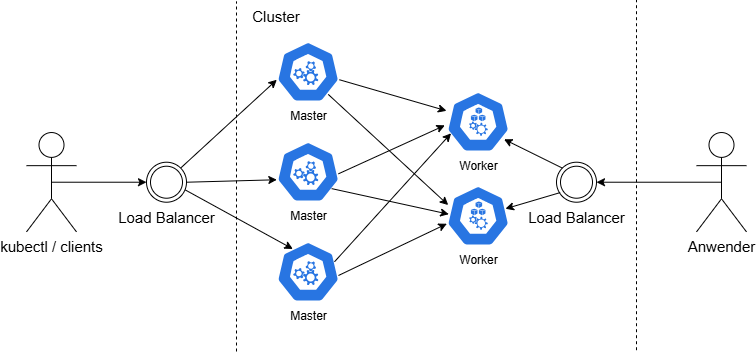
\includegraphics[width=0.8\textwidth]{bilder/implementierung/HAarchitektur.png}
\caption{High-Availability Architektur}
\label{fig:HAarchitektur}
\end{figure}

Das Ziel ist bei dieser Umsetzung einen Kubernetes Cluster mit einer HA Architektur im Hochschulnetzwerk einzurichten.
\FloatBarrier

\subsection{Verwendete Technologien/Werkzeuge}

\subsubsection{k3s}

Da der Production Cluster im Hochschulnetzwerk ohne Cloud-Einbindung betrieben werden soll, musste auf einen geringeren Ressourcenverbrauch geachtet werden.
Darüber hinaus benötigt Codetask aufgrund seiner überschaubaren Anzahl an Microservices aktuell noch keinen größeren Cluster.
Daher wurde sich gegen eine Standard-Kubernetes-Anwendung wie kubeadm oder Kubespray und für eine leichtgewichtige Kubernetes-Anwendung entschieden.

Dabei wurde die Entscheidung für K3s getroffen. Einerseits wurde ein k3s-Cluster parallel in einem anderen Projekt von Herrn Boger eingerichtet, andererseits bietet k3s auch darüber hinaus viele Vorteile.
Zum einen wurde k3s speziell entwickelt, um ein Kubernetes-Cluster in ressourcenbeschränkten Umgebungen auf Produktionsniveau auszuführen, beispielsweise auf IoT-Geräten.
Zum anderen hat k3s einen geringeren Einrichtungs- und Wartungsaufwand, da beim Installieren viele Komponenten, wie beispielsweise Traefik als Ingress-Controller, bereits integriert sind. Dadurch müssen weniger Komponenten separat installiert und konfiguriert werden.
Dadurch kann man sich mehr auf die eigentliche Anwendung konzentrieren statt auf die Clusteradministration.
Dennoch bleibt K3s einfach erweiterbar, unterstützt Hochverfügbarkeit, bietet eine gute Dokumentation und hat eine große Community.

\subsection{Umsetzung / Konfiguration}
Für die Einrichtung des Clusters im Hochschulnetzwerk hat die IT sechs VMs mit dem Betriebssystem Ubuntu bereitgestellt.
Auf einer der VMs wird der Load Balancer (LB) für die Verteilung der Anfragen zu den Master Nodes eingerichtet. Auf drei weiteren VMs werden die Master Nodes und auf den letzten beiden VMs die Worker Nodes eingerichtet.

Zunächst musste der Load Balancer eingerichtet werden. Dafür wurde auf der VM codetask-kub-lb HAProxy, ein Open-Source-TCP-LB, mit dem Befehl „sudo apt-get install haproxy” installiert.
Anschließend wurde die haproxy.cfg so erweitert, dass festgelegt wurde, über welchen Port der LB die Anfragen annimmt und wie er die Anfragen an die Master Nodes weiterleitet, um die Last zu verteilen.
Als Master Nodes wurden die IP-Adressen von codetask-kub-1 bis codetask-kub-3 angegeben.
Die Verteilung der Anfragen erfolgt über Round Robin, um die Last zu verteilen.

Nachdem der LB eingerichtet wurde, wird der Cluster gebootstrappt. Dazu wurde auf der VM codetask-kub-1 der folgende Befehl als HA Bootstrap gesetzt.
\begin{lstlisting}[language=bash, caption={K3s Installation mit HAProxy TLS-SAN}]
curl -sfL https://get.k3s.io | \
INSTALL_K3S_EXEC="server --cluster-init --tls-san <HAPROXY-IP>" sh -
\end{lstlisting}
Die Flag „--cluster-init” initialisiert den k3s-Cluster, während die Flag „--tls-san” den Zugriff über HAProxy ermöglicht.

Nach dem Bootstrap des Clusters nehmen wir den Token aus codetask-kub-1, um die VMs codetask-kub-2 und codetask-kub-3 als weitere Master-Nodes in den Cluster zu joinen.
Dafür wurde im folgenden Befehl, der auf beiden VMs ausgeführt wurde, dieser Token mitgegeben. Außerdem wurde angegeben, über welchen Server die VM den Cluster joinen muss. In diesem Fall ist es der HAProxy.
\begin{lstlisting}[language=bash, caption={Master Nodes joinen mit HAProxy TLS-SAN}]
curl -sfL https://get.k3s.io | \ 
INSTALL_K3S_EXEC="server --server https://<HAPROXY-IP>:443 --tls-san <HAPROXY-IP>" K3S_TOKEN=<TOKEN> sh -
\end{lstlisting}

Zum Schluss mussten die VMs „codetask-kub-4” und „codetask-kub-5” nur noch als Worker Nodes dem Cluster beitreten. Anders als bei Master Nodes muss dafür aber nicht explizit die Rolle angegeben werden.
Der Zugriff über den LB muss auch nicht erlaubt werden, da auf die Worker Nodes nur über die Master Nodes zugegriffen wird.
\begin{lstlisting}[language=bash, caption={Worker Nodes joinen}]
curl -sfL https://get.k3s.io | \
K3S_URL=https://<HAPROXY-IP>:443 K3S_TOKEN=<TOKEN> sh -
\end{lstlisting}
\subsection{Probleme und Anpassungen}
Das erste Problem, das bei der Umsetzung aufgetreten ist, betraf die Frage, über welchen Port der HAProxy erreichbar ist.
Normalerweise wird Port 6443 genutzt, da dieser bei Kubernetes-Nodes der lokale Zugang zu den Kube-APIs ist.
Der Port 6443 ist vom VPN aus jedoch nicht erreichbar, da es sich um einen administrativen Port handelt. 
Das verursacht keine Probleme zwischen VMs im gleichen Netz. Wenn jedoch außerhalb des Netzes über den VPN mit dem Cluster kommuniziert werden soll, ist dieser blockiert.
Deshalb wurde der Port, über den HAProxy erreichbar ist, von 6443 auf 443 geändert.

Ein weiteres Problem ergab sich, da die vorhandenen Worker Nodes im Cluster bei der Reaktivierung ständig selbst auf „notReady” gestellt wurden.
Die Ursache des Problems war, dass die Worker Nodes mit dem Cluster verbunden wurden, aber die Umgebungsvariablen K3S\_TOKEN und K3S\_URL in der Konfiguration fehlten.
Um das Problem zu lösen, wurden die Umgebungsvariablen manuell in der Konfiguration nachgetragen, wodurch die Worker Nodes stabil im Cluster wurden.
\subsection{Ergebnisse der Umsetzung}
Durch die Umsetzung gibt es ein k3s-Cluster mit HA-Architektur für die Produktionsumgebung im Hochschulnetzwerk. 
Da die Anwendung im Hochschulnetzwerk bleibt, müssen die VMs nicht über Tools wie OpenTofu und Proxmox selbst verwaltet werden, sondern weiterhin von der IT.
Der Cluster kann per SSH auf einen Master-Node zugegriffen werden. Es gibt aber auch die Möglichkeit, einen Admin-Rechner einzurichten. Dieser kann über den LB auf den Cluster zugreifen. 
Das ist praktisch, wenn es benötigt wird, bei einen größeren Betrieb.

Diese Ergebnisse steigern die Zuverlässigkeit. 
Dank der HA-Architektur hat die Anwendung nicht nur eine höhere Verfügbarkeit, sondern auch eine bessere Fehlertoleranz. So können nicht nur Ausfälle von Worker Nodes, sondern auch von Master Nodes toleriert werden.
Durch den Load Balancer und die mehreren Master- und Worker-Nodes steigt auch die Stabilität der Anwendung, da diese ihre Last nun besser verteilen kann.

Hinzu kommt, dass dieses System skalierbar ist. Wenn bei einen größeren Betriebsverhalten mehr Last erzeugt wird, können weitere Master- und Worker-Nodes zum Cluster hinzugefügt werden, um diese besser zuverteilen.
Auch der LB kann Replicas bekommen bei einen Wachstum der Nodes. Daher kann der Cluster mit Codetask zusammen wachsen.

